\section{In the gm2 Framework}

  Depending on the level to which a user wants to utilize or develop the tracking code, they may choose which branches of the gm2 framework to checkout. If just fitting tracks and viewing plots, then just gm2tracker on the develop branch may be checked out. If doing further development, it can be a good idea to checkout the artg4, gm2dataproducts, gm2geom, gm2ringsim, gm2tracker, and gm2utils packages of the gm2 repository, and be on the feature/trackDevelop branch in all instances. Every so often these branches are merged with the main develop branches, where the tracking code will work but might not have the latest code changes. 

  \subsection{Event Generation, Geometry, and Material}

    While not a direct part of the reconstruction and fitting code, there is relevant information with respect to event generation in the simulation upon which the reconstruction acts. Event generation before fitting is done using the mdc fcl files in gm2ringsim using the main simulation, where one can also include the tracker dummy plane geometry for truth comparison with the Geane fitting if so desired. These are built in the TrackerDummyPlane\_service and associated geometry files, and are included in the common mdc fcl files. If one wishes there are also a couple of modified mdc\#-geane fcl files available for use with reduced geometry. For stats reasons it is usually a good idea to include all 3 trackers when generating events.

    Fcl parameters exist for the StrawTrackerCadMesh\_service and Straws\_service in order to turn material on or off at will, ``materialTracker'' and ``strawMaterial'' respectively. The rest of the geometry has to be manually changed and rebuilt in order to remove material if one wishes. These include VacuumChamberCadMesh and the World, as well as the ``buildSupportPost'' option in strawtracker.fcl, ``buildTrolly'' in vac.fcl (where the associated material is hardcoded in), and ``trolleySupportMaterial,'' also in vac.fcl. One should make sure to perform reconstruction with the same material parameters as were used in the event generation for proper results. (These options are primarily for debugging the tracking. Near perfect results have been shown for tracking within a vacuum world, \href{http://gm2-docdb.fnal.gov:8080/cgi-bin/ShowDocument?docid=4876}{DocDB 4876} and \href{http://gm2-docdb.fnal.gov:8080/cgi-bin/ShowDocument?docid=4894}{DocDB 4894}.)


  \subsection{Reconstruction Flow}

    The overall tracking infrastructure and reconstruction flow can be seen in Figure \ref{fig:Infrastructure}. Data coming from simulation or the real experiment, are turned into art objects upon which the tracking framework acts. The RunGeane.fcl file (detailed more below) performs the entire chain within the blue box in Figure \ref{fig:Infrastructure}, excepting the track extrapolation stage. Within the reconstruction flow objects called Track Candidates are produced, which are the input to the Geane fitting code.


\begin{figure}[]
\caption{Shown is the infrastructure flow for the entire track reconstruction chain. In the green blocks are the sources of track data to fit, either from Geant simulation, or real data. In blue is the offline reconstruction block. Straw digits are formed in the digitalization step, those are then calibrated and grouped into time islands, clusters, and seeds which then combine to form track candidates. It is these track candidates which are the input into the Geane fitting code (and other future fitting code). The fitting code then outputs tracks which the track extrapolation stage will run over. This picture is taken from one of Tammy's talks. Note that there is some iteration here that is not shown.}
\centering
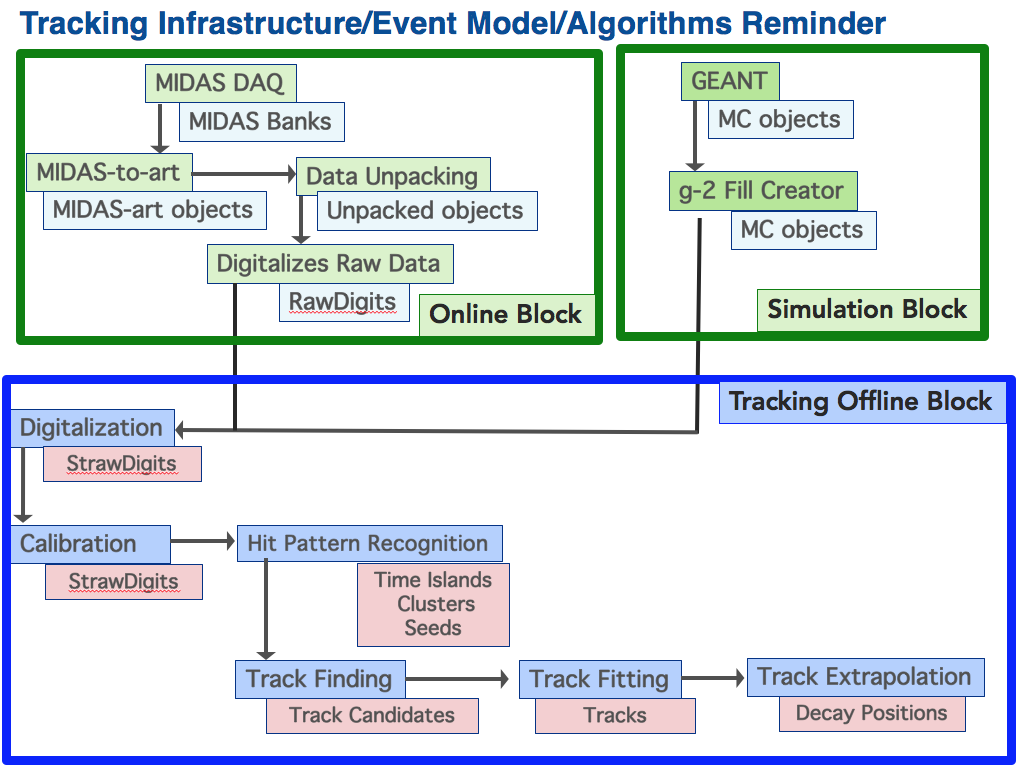
\includegraphics[width=0.9\textwidth]{TrackInfrastructure}
\label{fig:Infrastructure}
\end{figure}

\begin{figure}[]
\caption{Shown is the Geane fitting code flow. See the text for a thorough explanation of this flow, and the specifics of each box. GEANEArtRecords are created in the GeaneReco producer module, and are passed by pointer and reference to the different utils files which then updates them for the different fitting modes and with the fitting results.}
\centering
\hspace{15mm}
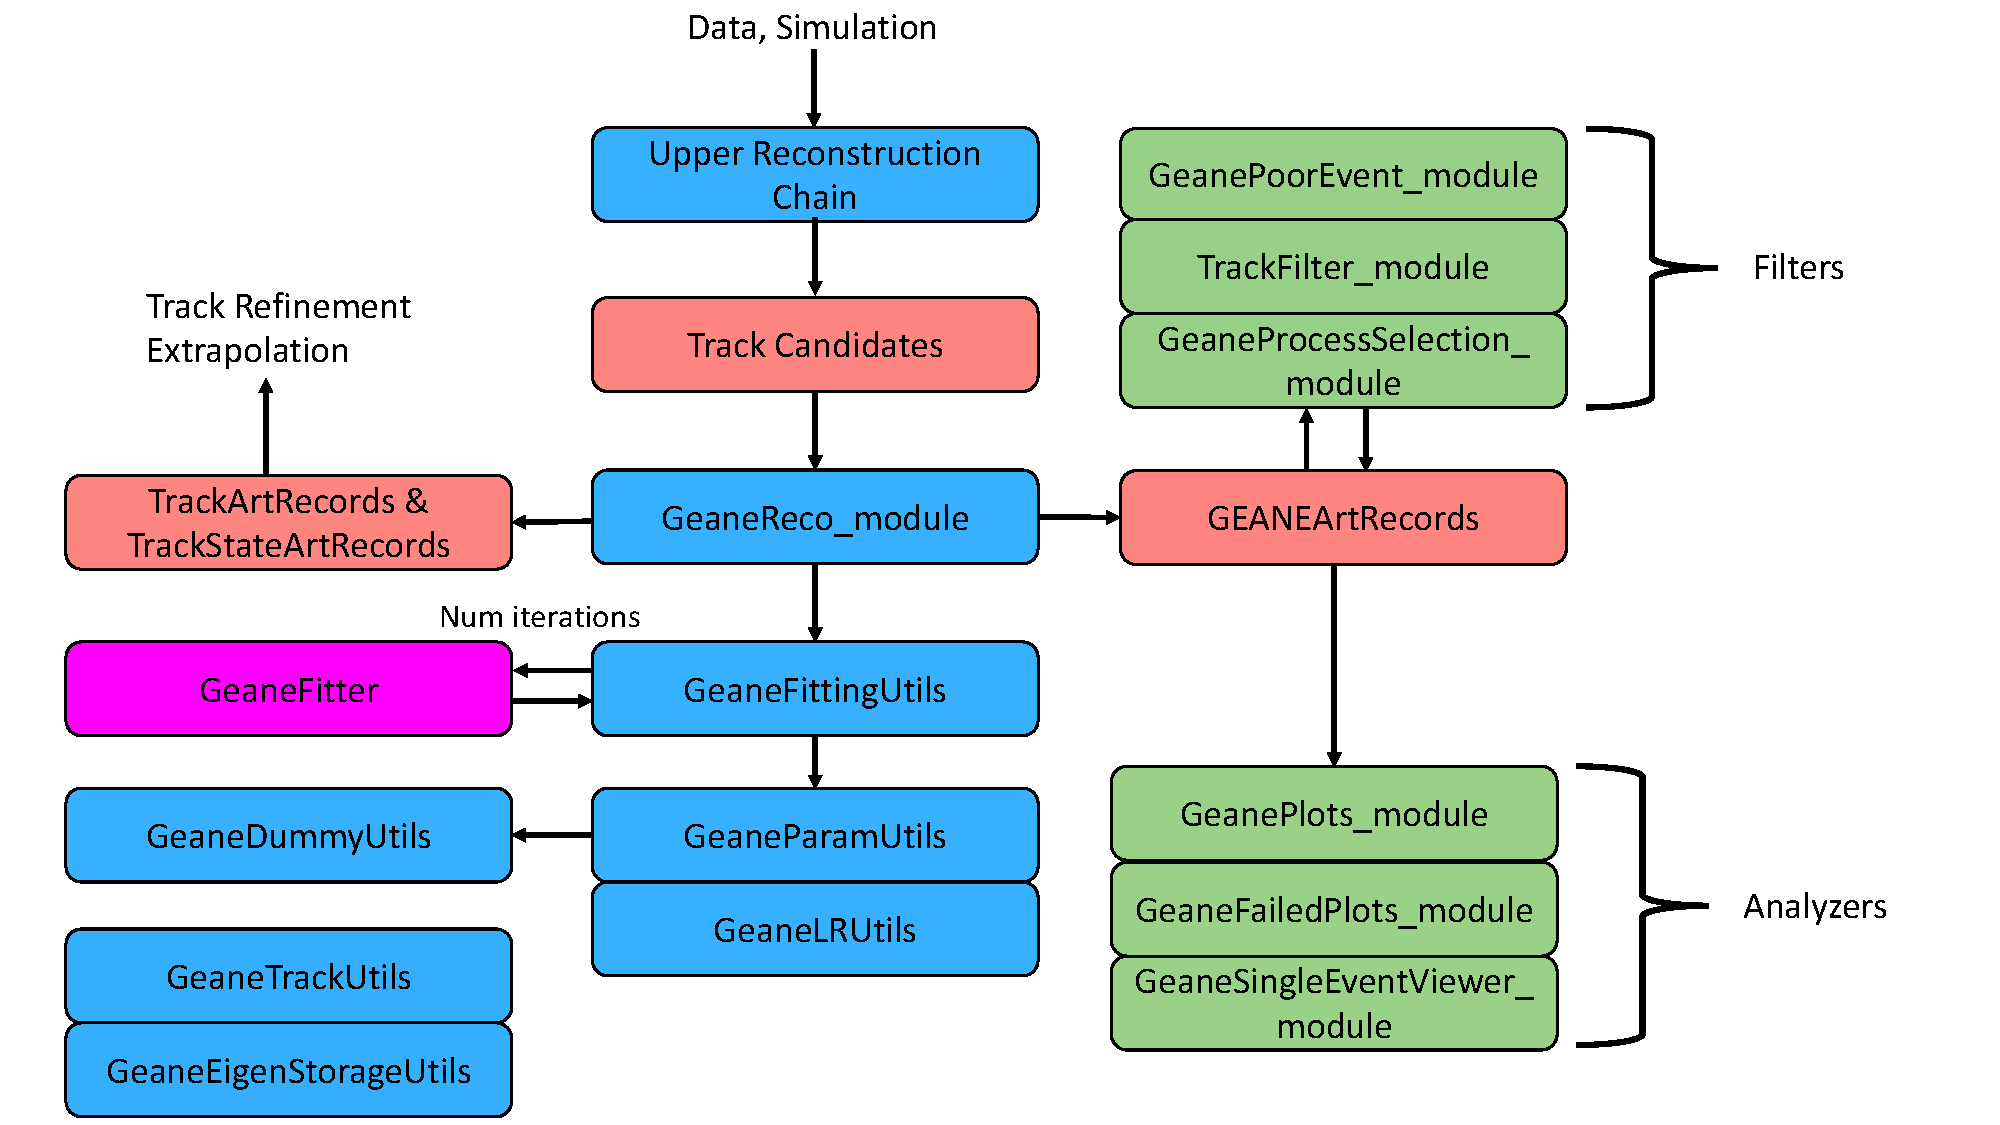
\includegraphics[width=0.9\textwidth]{NewGeaneFlow}
\label{fig:NewGeaneFlow}
\end{figure}


    The Geane fitting specific flow can be seen in Figure \ref{fig:NewGeaneFlow}. There is a number of files involved in the production of fitted tracks. Detailed information regarding all of these files is given below, but here is provided a shorter summary. Track candidates from upstream are used as the input to the producer module GeaneReco, which produces TrackArtRecords and TrackStateArtRecords, which are then passed to the extrapolation or refinement stage. GeaneReco also produces GEANEArtRecords, which is the data product that is used and updated throughout the fitting process until the track converges or fails, and may be passed through filters or to analyzers at the end of the fitting. There are a number of utils files that the Geane fitting utilizes. GeaneReco directly links to the GeaneFittingUtils which contains a number of methods for the different fitting modes, as well as the general fitting loop which links to the GeaneFitter class, and iterates until the track fitting succeeds or fails. GeaneFitter provides a $\chi^{2}$ and improvement to the track as described in the \hyperref[sec:Formalism]{Formalism} section. GeaneFittingUtils links to GeaneParamUtils and GeaneLRUtils. GeaneParamUtils deals with any code that modifies parameters regarding the fit, both setting up the initial fit parameters, and calculating the predicted parameters of the fit within Geant4 using the error\_propagation routines. GeaneLRUtils deals with any code regarding the left and right information of the track for fitting.
    
    Note that after a single iteration, one pass through GeaneFitter and one pass through the relevant fitting utils, a $\chi^{2}$ and an improvement for the track will be produced, but the track predicted parameters and objects will be based on the previous starting position and momentum guess before it has been updated, and so do not correspond to the fitted track. It's necessary to perform at least a second iteration for this reason, and is why no track converges under the strict criteria in under 3 iterations.

    Also worth mentioning is that the GEANEArtRecords are passed by reference or pointer throughout the various fitting files, allowing them to be updated along the way in a natural manner. At the same time, many methods within the fitting code return ints describing whether the track fitting has failed at different stages to various reasons, where a value of 0 signifies success at that stage. A returned int with a non-zero value might for example signify that too many digits were included in the initial track candidate, or that Geant is having tracking issues, etc.


  \subsection{fcl File Specifics - RunGeane.fcl} 

    Reconstruction is performed using RunGeane.fcl in gm2tracker on the events generated from somewhere higher in the chain. (There is also a RunGeane-midasdata.fcl file which is more tuned to running on real data, with certain fcl parameters set appropriately and some modules left out of the chain.) It is important to explain some fcl parameters necessary for the reconstruction. First, there is a fcl parameter ``useSD'' for the Straws geometry service to turn off the straw sensitive detectors so that in the reconstruction phase hits are not regenerated. If this is not included, it will default to true and cause crashes in the reconstruction. Secondly, the RunGeane.fcl file loads all 3 trackers necessary for symbol and name definitions, but such that tracker 0 (or 18) is rotated such that the tracking planes are parallel to the global geant X axis (using the rotateArcTracker fcl parameter for the Arc service). This is done to avoid the issue of error propagation instability close to the Z axis, as detailed in \href{http://gm2-docdb.fnal.gov:8080/cgi-bin/ShowDocument?docid=4567}{DocDB 4567}, while at the same time still observing the correct azimuthally symmetric 2D field for the tracks. Track hits are rotated from their separate tracker frames to this one reconstruction frame with the GeaneWorldTracker[0], GeaneWorldTracker[12], and GeaneWorldTracker[18] transforms defined at the bottom of StrawTrackerCadMesh\_service.cc, and as detailed in the \hyperref[sec:Coord]{Coordinate Systems} section. (In the future, if fields or geometries are not identical between trackers, the details here will have to be improved after changes have been made.) As a reminder there are material fcl parameters for the straws and straw trackers which should be the same as were used in the event generation. The RunGeane.fcl file also includes some analyzer and filter modules by default, which are detailed further below, and can be turned on and off at will.

    While the pieces of the chain before the track fitting (digitalizing, seeding, clustering, t0 finder, and track finding) are distinct and separate from the material detailed in this document, it is important to understand at some level those stages and the different options which will affect the tracking results. See a collaboration talk by Tammy, \href{http://gm2-docdb.fnal.gov:8080/cgi-bin/ShowDocument?docid=5601}{DocDB 5601}, for a general overview on this. Here is a short summary, not all method or file calls are detailed. Most of these files and parameters should be left unchanged unless one is familiar with the subject matter.

    \begin{enumerate}

          \item{\bf{Digitalizer\_module.cc}} \\
          This module creates StrawDigits which will ultimately be combined to form the Track Candidates that the fitting will act over. It is the variables in this art record that are updated and correspond to real data, which straw was hit, the time of the hit, and the dca of the hit. The StrawDigits also contain a pointer to a struct of Monte-Carlo truth data, StrawMCDigit, which can also be accessed for track information. The Digitalizer module has several fcl parameters to change things like the gas drift time, drift model, allowing recorded negative times, and some particle cuts. By default it uses a Gaussian drift model which is called when the Digitalizer calls the DriftTimeModels.cc file, where it will gaussian smear the hit time from the MC digit time. These fcl parameters are located in digitalizerParams.fcl. The smearedDriftTimeSeed parameter should be set to 0 if one wants random results from run to run, which is necessary for grid jobs. The drift time model can also be set to the Garfield version, which will produce more realistic measurement parameters. If this is used the drift time calculator in the DriftDistanceCal module should also be set to the Garfield version. These more realistic hit data result in reconstructed tracks that haven't been fully analyzed yet, with a non-uniform p value distribution.

          \item{\bf{TimeIsland\_module.cc}} \\
          Groups the digits from the Digitalizer in time. Has some options for changing the time window width. fcl parameters are located in recoIslandParams.fcl. There is ongoing work in relation to this module for dealing with real data, where there is a much increased number of hits closer in time. The short summary here does not reflect the difficult and important task that this module has.

          \item{\bf{ClusterFormation\_module.cc}} \\
          Groups neighboring digits in the same view to form clusters. fcl parameters are located in recoClusterParams.fcl.

          \item{\bf{T0Finder\_module.cc}} \\
          Calculates a t0 for the track. Has an option for which model to use for calculating said t0. The default is using truthData if one is running the tracking over simulated hits. If one is looking at real data there are other options. It's important to note that the t0 for a track can be difficult to calculate, and the current goal is to combine information from the calorimeter to get this number. fcl parameters are located in recoT0FindingParams.fcl.

          \item{\bf{DriftDistanceCal\_module.cc}} \\
          Calculates the drift times and distances within the straws based on the calculated t0 from the previous module. Has options for different drift calculators and parameters, including a ``useTrueDigitT0'' parameter for using mc truth information. The drift time is calculated from the digit hit time (calculated in the Digitalizer) minus the digit t0. If true t0 is not used, then the dca smearing will not be perfectly gaussian. fcl parameters are located in recoClusterParams.fcl.

          \item{\bf{SeedFormation\_module.cc}} \\
          Groups neighboring clusters in the same module to form seeds. There are two fcl parameters for this module. The first is ``reconstructPosition'' which will fill seed nodes which form the seed, and essentially correspond to indidual digits - but which contain some left-right (LR) ambiguity information important for track fitting. The second is ``useGeometryLR'' which uses the straw geometry information to make an initial guess at the left-right choices for doublets within the track. fcl parameters are located in recoSeedParams.fcl.

          \item{\bf{Aside}}
          It's important to note that there is another iteration of the clustering module which is improved now that better drift times and distances have been calculated from the previous modules, using the same fcl paramters. This will almost certainly change in the future as the tracking code becomes more developed.

          \item{\bf{TrackFinding\_module.cc}} \\
          Groups time islands and digits based on their positions in space. There are two finders available for use, fcl parameter trackFinderName, the Simple Track Finder (SimpleTrackFindingUtils.cc) and the Long Track Finder (LongTrackFindingUtils.cc). The former just runs off the generated time islands. If you use this, then the second clustering module and seed formation module can be left out of the reconstruction chain. The latter, Long Track Finder, forms track candidates based on combining seeds and is the default used. It also has stricter fcl conditions, such as a default cut of 6 or more planes hit for the track. Both finders make use of the SimpleCircleFitter.cc class which fits a circle to the U and V digit positions to calculate a starting position and momentum guess for the track, which is currently necessary for the Geane fitting. The Long Track Finder also has a least squares minimizer which is unimportant for the Geane fitting. fcl parameters are located in recoFindingParams.fcl, which then also links to some other fcl files depending on the finder used.


    \end{enumerate}

  \subsection{geaneFitParams.fcl}

    Because the Geane track fitting is the subject of this document, it will go more into detail of the Geane fitter fcl parameters, located in the geaneFitParams.fcl file. Some of these parameters are very likely to change or disappear in the near future.

    \begin{enumerate}

      \item{\bf{module\_type}} \\
      The ordinary art producer parameter which tells art which cc file to run, this is always set to GeaneReco unless the filename changes.

      \item{\bf{G4EVERBOSE}} \\
      This parameter corresponds to the iverbose level present in the Geant4 error\_propagation files and can be manually set here, from 0 to 5. It is for the debugging of deeper level Geane fitting code. Note that unless Geant is compiled with the flag by the same name setting this verbose level will do nothing. Since currently we utilize our own slightly modified error\_propagation files copied into the gm2tracker/gm2Geane directory, it would be possible to remove the dependencies on this Geant4 build flag. Since however this will slow down the tracking it is the current choice to leave them in. 

      \item{\bf{trackingVerbose}} \\
      Geant4 tracking verbose level, from 0 to 5. This is always available but should only be used for debugging.

      \item{\bf{matrixDebug}} \\
      This boolean paramater turns on and off the copious matrix debugging output, used for deep level debugging. Note that these outputs are included in the log file and the log file threshold needs to be set to ``DEBUG''. In the future it might be beneficial for speed reasons to remove completely these debugging outputs. This parameter should always be turned off if looking at a large number of events.

      \item{\bf{numPassesWireFit, numPassesSeqFit}} \\
      These are parameters used for the Left-Right sequence checking routines for a full fit. numPassesWireFit is the number of passes that the track should be fit to the wire centers, before which the best sequences were passed to the main fit code which would iterate a number of times equal to numPassesSeqFit. It was observed in the past that 3 passes for each of these was sufficient for good tracking results. 

      \item{\bf{convergenceCriteria}} \\
      This is a scalar convergence criteria telling whether the track fitting has been successful or not, with a default value of .1. As long as the current iteration $\chi^{2}$ minus the previous iteration $\chi^{2}$ is less than this value, the track is considered to have converged, otherwise it continues iterating until it succeeds, fails, or is manually cut off at 10 iterations.

      \item{\bf{useCircleGuess}} \\
      This boolean parameter tells the code whether to use the circle fitter results for the track starting guess or not, called in the track finding part of the chain. It's default should remain true unless one wants to return to the uniform starting parameter smearing for debugging purposes.

      \item{\bf{lockLowDCAs}} \\
      This is a temporary fcl parameter which will take measured hits with small dcas and set the measured positions to the wire centers, at the same time locking the LR choices to the center. This will be necessary when fitting data due to the large measurement uncertainty of hits close to the wire, and at the same time speeds up the code with less LR choices to iterate over. It's default value of 0 corresponds to turning this functionality off, while a positive number corresponds to the radius in mm that dcas less than will be locked.

      \item{\bf{useNodes}} \\
      This boolean parameter sets whether to use the left-right information from the seed nodes, if activated. The recoSeedParams fcl parameter ``reconstructPosition'' needs to be set to true for this to work, and the parameter ``useGeometryLR'' should also be set to true, being that it is the only upstream left-right code currently implemented.

      \item{\bf{fitMode}} \\
      This is the most important fcl parameter for the Geane fitting. It defines what type of fitting mode you'd like to use for fitting the incoming track candidates. There are currently 4 separate fitting modes. ``truthLRFit'' only works with simulated data and will fit to the unambiguous LR UV values from the digits. ``wireFit'' will fit a track to the wire centers of the incoming digits, with a corresponding uniform error proportional to the gas diameter. ``mainFit'' will first do a wire fit to the track in order to make an initial guess at the LR choices for each hit, and will then fit to those LR choices. (The default main fit actually does a second wire fit in the middle where it first locks LR choices for doublets where the LR choice is guaranteed to be known, which improves the tracking results slightly.) Finally there is the ``fullSeqFit'' which will first do the wire fit, and will then go about checking all LR sequences before doing full fits on the set of best sequences. (There is also some code to lock the left-right sides based on the doublets.) This LR procedure is detailed lower in this document.

      \item{\bf{useTangentLR}} \\
      This fcl parameter links to code which does a slightly more advanced locking of the doublet left-right geometry include track tangent information, defaulted to false, and written by Joe Price.

      \item{\bf{rseed, yPosChange, zPosChange, xMomChange, yMomChange, zMomChange}} \\
      These are the uniform smearing bounds for the starting position and momentum of the track from truth, units of mm and MeV. These are largely unused now since the circle fitter provides a level of smearing automatically when it's used, but should be kept for future debugging purposes. The rseed parameter is the number seed for the random number generator. The default should be 0 for the root TRandoms unless one wants to reproduce results.

    \end{enumerate}


  \subsection{Reconstruction Files}

    Here will be given a summary of the different core files used in the Geane track fitting as shown in Figure \ref{fig:NewGeaneFlow} and explained up above, as well as extensive detail where necessary. 


    \begin{enumerate}

      \item{\bf{GeaneReco\_module.cc}} \\
      This file is the producer module for the track fitting reconstruction. It pulls in upstream data products, TrackCandidateArtRecords, and produces TrackArtRecords, TrackStateArtRecords, and GEANEArtRecords. The GEANEArtRecords are what's passed through the various fitting utils files until the track fitting succeeds or fails, and from which the TrackArtRecords and TrackStateArtRecords are derived from. GeaneReco directly links to GeaneFittingUtils where the track fitting is actually done.

      \underline{Methods}

        \begin{itemize}

          \item{\bf{produce}} \\
          General overriden produce method. Calls main track fitting code on an event by event basis. Produces data products for downstream use.

          \item{\bf{trackFitting}} \\ 
          Short method which first calls down through GeaneFittingUtils into GeaneParamUtils to set up the initial parameters for fitting, and then calls the method corresponding to the particular fit mode specified in the fcl file. Also has a method call for checking some failure modes after fitting.

        \end{itemize}

      \item{\bf{GeaneFittingUtils.cc}} \\
      \label{sec:GeaneFittingUtils}
      This class contains several methods for fitting tracks with different fit modes. Each such method sets up the specifics of the fit, altering necessary parameters and calling various methods, and then calling the fittingLoop method which iterates and fits the track. mainFit and fullSeqFit do multiple fits, starting with a wire fit. 

      \underline{Methods}

        \begin{itemize}

          \item{\bf{truthLRFit}} \\
          Fits a track to the U and V hits with the left-right sides known from the Monte Carlo simulation. Only works with simulation.

          \item{\bf{wireFit}} \\
          Fits a track to the wire centers of the hit straws, ignoring left-right information. This is the easiest fit to do on data since it ignores timing information, which affects dca values and errors.

          \item{\bf{mainFit}} \\
          First does a wire fit to the track in order to gain left-right information, then does a hybrid wire fit with some left-right choices set based on the doublet geometry and predicted parameters from the first wire fit. Finally fits a track to the dca values of the hits with the left-right sides set from the previous fit, updating each iteration.

          \item{\bf{fullSeqFit}} \\
          First does a wire fit to the track in order to gain information useful for solving for the left-right sides of the track. Then locks left-right sides based on used fcl parameters, and sets associated errors, leaving the remaining sides as ``unknown.'' Then does a fast check or approximate fit on all U and V unknowns separately in order to determine a set of best possible U and V left-right combinations. Finally takes the best U and V left-right combinations and combines them into full left-right sequences, which are then fitted as normal with the associated dcas and errors. See the \hyperref[sec:LR]{Left-Right} section for more detail on this.

          \item{\bf{fittingLoop}} \\ 
          The general fitting iteration loop method. Takes in the GEANEArtRecord, the number of passes to fit over, and whether to update the left-right sides each iteration (for mainFit) as parameters. For each loop it will calculate the predicted parameters and propagate the errors of the fit by calling the errorProp method within GeaneParamUtils, then update the left-right sides from the previous iteration if desired, then calculate the angle-corrected measured parameters based on the left-right sides of the track to fit. Finally, with all parameters determined, it will calculate a $\chi^{2}$ and an improvement for the track by calling the TrackCorrelation method from the class GeaneFitter. The improvement to the track from GeaneFitter serves as the basis for calculating the next set of predicted parameters. Relevant GEANEArtRecord members are filled and then the track is checked to have converged, with fittingLoop iterating if it has not. 

          \item{\bf{checkExtraneousFailureModes}} \\
          A mostly defunct method with the purpose of checking to see whether the tracking has failed in some unseen way. In the past there were some failure modes which have since been removed such as a track reconstructed with overly high momentum. Currently the only failure mode check is to see whether the X positions of the reconstructed track don't match the wire positions, which should not be the case since the former directly comes from the other. Some coordinate code which may be the root cause of this is commented out due to framework coding constraints (which can probably be gotten around). This method has been left in for the future possibility of checking other potential failure modes.

        \end{itemize}

      \item{\bf{GeaneFitter.cc}} \\
      This file consists of the main track fitting $\chi^{2}$ algorithm. It multiplies measured parameters, predicted parameters, error matrices, and transport matrices together to produce a chi2 for the track and an improvement to the starting paramters. It also reads in the measured hits errors in order to properly fit the track. See the \hyperref[sec:Formalism]{Formalism} section for a detailed description of what this class really does. There is a fcl parameter matrixDebug which can be used to turn on or off the many large matrix cout debugging statements.

        \begin{itemize}

          \item{\bf{TrackCorrelation}} \\
          The main matrix multiplication routines, essentially the math from reference \cite{geanemanual}. In order to fit the track properly with the correct errors, the matrix multiplication must be done in the XUV space. Since the transport matrices and predicted parameters are generated in the XYZ space as described in the errorProp method of the \hyperref[sec:GeaneParamUtils]{GeaneParamUtils} section, they must be converted using the Jacobian transformation between the two bases. This Jacobian is described in the \hyperref[sec:Coord]{Coordinate Systems} section, and the variable itself is saved as a member in the GeaneTrackUtils.cc class. 

          One other point of note regarding this method is that depending on the matrix multiplications being done, the various loops within the code might either loop over the maximum number of planes (33, a 0 plane plus the 32 measurement planes), or they might loop over the planes that were hit. The code should be relatively clear, but if any indices or loop iterators are messed up in any way, then the track fitting will utterly fail, sometimes with only very subtle hints as to where exactly the problem lies. (At one point I spent a week hunting down an off-by-one index error believing it to be a memory problem, due to how the Eigen matrices work.) At some point it might be beneficial to standardize this code, but it has been left alone per the reason stated before.

          \item{\bf{makeHybridErrMat}} \\
          A method in order to create a hybrid wire / U or V error matrix for the left-right sequence checking. Only called once per track for the U and V sequences.

          \item{\bf{sequenceChecking}} \\ 
          The main left-right sequence checking method for an individual event. This method is called up to thousands of times as each U or V sequence is checked. See the \hyperref[sec:GeaneLRUtils]{GeaneLRUtils.cc} and \hyperref[sec:LR]{Left-Right} sections further below for more detail on what this method does.

          \item{\bf{convertToGeVcm, convertToMeVmm}} \\
          Methods for converting Eigen 5 parameter vectors from GeV cm to MeV mm and vice versa.

        \end{itemize}

      \item{\bf{GeaneParamUtils.cc}} \\
      \label{sec:GeaneParamUtils}
      This file consists of the main methods which modify various parameters for the track fitting. The setupParams method does its namesake, setting up the initial parameters per track before attempting to fit. The errorProp method deals with calculating predicted parameters and associated track matrices within Geant4. Finally, the calcMeasuredParams method deals with setting and correcting the measured paramaters of the fit from the incoming dca values and errors of the track hits. Note that this is the only class in the Geane reconstruction framework which links to and uses Geant4. It is in the constructor of this method that the Geant4 world is constructed once per job, the proper magnetic field is associated with the transportation manager, and the error propagation routines are initialized. (The necessary Geant4, art service, and gm2geom header files are included here.)

      \underline{Methods}

        \begin{itemize}

          \item{\bf{setXPositions, setCoordMap}} \\
          Hacked in methods to grab needed coordinate system information and the X positions of the wire planes (from the art run object) while improving speed of the tracking.

          \item{\bf{setupParams}} \\
          This method sets up the parameters at the beginning of each track fit. It is here that the TrackCandidateArtRecord and StrawDigitArtRecord information is copied or converted into relevant GEANEArtRecord members. Other members are filled with default or empty values to start. Members include dcas, dca errors, wire positions, hit sides, etc. This method links to the GeaneDummyUtils file, which allows one to acquire the truth information of the track and use for fitting if desired. The starting guess for the position and momentum of the track can be pulled from the track candidate (calculated using a simple circle fitter to the hit digits) or truth. There are a couple of variables in the GEANEArtRecord which are filled with the same information in this method, as the initial setup is for doing a wire fit to the track. If doing a different kind of fit, the variable changes and method calls in GeaneFittingUtils handles altering the relevant parameters of the fit. There are also a couple of checks in this method to make sure that we're trying to fit a reasonable track, and not one that for instance has more than one hit on a measurement plane.

          \item{\bf{errorProp}} \\ 
          This method tracks particles along their average trajectories through the region of the tracker detector using the Geant4 error propagation routines with the correct geometry and field. It builds transport matrices, error matrices, and predicted parameters which are the objects used for fitting the track, as described in the \hyperref[sec:Formalism]{Formalism} section. It tracks on a plane by plane and step by step basis. These error propagation routines can be used to track particles forwards and backwards, where the forwards tracking is used in the code. (It will be non-trivial to change the code to be able to back-track.) 

          To be a little more explicit, it creates Geane free trajectory states which are the objects that are propageted from target plane to target plane, where the target planes are defined to be parallel in X. (As our wire planes are.) Surface trajectory states are then created on those planes, where the orthonormal vectors defining those planes are in the Y and Z directions. These vectors have to be orthornormal in Geant in order for predicted parameters and errors to be calculated correctly. It is later in the fitting code that these track objects are converted to the UV basis that our detector is naturally defined in. 
            
          While the predicted parameters and errors can be grabbed directly from the surface trajectory state on each plane, the transport matrix cannot be. It is on a step by step basis that the transport matrices are generated, with the previous step transport matrix being dropped with the next step. It is for this reason that the transport matrices must be accumulated and multiplied together from each step in order to form the transport matrix describing the change in parameters from one measurement plane to the next. (There is some code in the Geant source code which appears that might do this automatically, but it is commented out and unclear if it works.) These transport matrices are also only defined in the free state coordinate system, and so need to be converted to the surface system that our fitting uses. When creating surface trajectory states on the target planes, the Jacobian transformation matrices from the free to the surface system are generated and can be saved. It is then a simple matter of multiplying these matrices together to get the transport matrices in the surface system. (Once again these are defined in XYZ, but are converted later in the code to be in XUV.)

          Transport matrices are accumulated as
              \begin{align} %\label{eq:nolabel}
                T_{mn} = T_{mk}T_{kn},
              \end{align}
          where the indices can stand for either plane numbers or step numbers, and converted by 
              \begin{align} %\label{eq:nolabel}
                T_{mn,s} = A_{n} T_{mn,f} A_{n}^{-1},
              \end{align}     
          where the indices s and f stand for the surface and free trajectory states respectively, and A is the Jacobian transformation from the free state to the surface state. See reference \cite{jacob} for the calculation of these Jacobians. The error matrices in the surface state can be grabbed directly from the Geant code unlike the transport matrices, or if necessary can be converted as
              \begin{align} %\label{eq:nolabel}
                \sigma_{m,s} = A_{m} \sigma_{m,f} A_{m}^{-1}.
              \end{align}   

          It's also worth mentioning that within this method there are a number of checks to see whether the tracking has failed due to Geant stepping or Geane propagation issues.

          \item{\bf{calcMeasuredParams}} \\ 
          Method to correct measured parameters from a radial DCA value to a U or V value based on the momentum of the track at the hit from the previous fit and approximating a constant field within the straw. Also corrects the dca errors using a simple straight line approximation in a similar vein. See the \hyperref[sec:Appendix]{Appendix} section for more details on how this works. Note that this method also fills the measured parameter objects within the fit in the first place, so if this method is not called then the fit won't have any measured hits to fit to.

        \end{itemize}

      \item{\bf{GeaneDummyUtils.cc}} \\
      This class deals with truth track information, stored in GhostDetectorArtRecords generated by the TrackerDummyPlane service. These GhostDetectorArtRecords store position and momentum in the world coordinate system, and so need to be converted to the Geane coordinate system(s) when comparing the fitted track against truth or inputting any truth parameters into the fit. Called by GeaneParamUtils and some analyzers.

      \underline{Methods}

        \begin{itemize}

          \item{\bf{fillDummyHits}} \\
          Fills a local variable with the dummy hits from the art data handle, done once so that the utils file has access to the data products.

          \item{\bf{getTrackDummyHits}} \\
          Method to fill the GEANEArtRecord dummy hits member variable, dummyPlaneHits, with the ordered dummy hits corresponding to the hit measurement planes.

          \item{\bf{fillCS, fillStationStr}} \\
          Passes some needed coordinate system information to the utils file, and the station that the track was in for coordinate transforms to the correct frame.

          \item{\bf{fillDummyHitInfo, fillDigitHitInfo}} \\
          Fills some commonly used variables throughout different methods in the class.

          \item{\bf{fillTruthParams}} \\
          Brute force searches through the GhostDetectorArtRecords to find the hits corresponding to the digits in the track, and sorting them before calling the getTrackDummyHits method. This is kind of an awkward method because the GhostDetectorArtRecord can't store any sort of plane or module identifiers, except for the volume string. These volume names have the form TRACKERDUMMYPLANEPV[a][b][c], with a the scallop number {0, 12, 18}, b the module number {0, 7}, and c the plane number {0, 3}. There are also ``0'' planes in front of each module for recording the ``starting'' positions of the tracks, defined as being 10 mm (by fcl parameter) in front of the first wire plane of each module. For these 0 planes, c equals 5. It is then a matter of looping through the GhostDetectorArtRecords until the indices and particle ID match the straw digit that was hit and storing those hits into a sorted member variable. There is associated logic to check all of these conditions, and it's not optimized.

          \item{\bf{createStartGuess}} \\
          If desired, this method can be called to create an intial start guess for the momentum and position from the truth information directly. This guess can be smeared variably with the associated fcl parameters if one wishes.

          \item{\bf{fillLRFromTruth}} \\
          This method calculates the true hit sides of the tracks using the GhostDetectorArtRecord positions and the wire information. These true hit sides can then be grabbed by GeaneParamUtils if one wishes to fit to truth, or the final left-right sides can be compared to the truth at the analyzer stage.

          \item{\bf{checkLRAgainstTruth}} \\
          This method checks to see how well the fitting fared when calculating the left-right sides of the track.


        \end{itemize}

      \item{\bf{GeaneLRUtils.cc}} \\
      \label{sec:GeaneLRUtils}
      This class deals with the left-right aspects of the Geane fitting. It has a couple of methods for functionality regarding hits with small dcas where the error on the hit is large, filling the left-right sides from upstream, the geometry, or the previous fit iteration, and finally a number of methods for different fitting steps within the full sequence checking left-right fit, fullSeqFit. See the fullSeqFit paragraph in the \hyperref[sec:GeaneFittingUtils]{GeaneFittingUtils} section for a quick description of how it works, and the \hyperref[sec:LR]{Left-Right} section for a more detailed description on how fullSeqFit works.

      \underline{Methods}

        \begin{itemize}

          \item{\bf{lockSmallDCAErrors, lockSmallDCACenters}} \\
          For hits with small dcas below some threshold, sets the fit errors accordingly, and the hit sides to the wire centers. The lockSmallDCACenters method takes as input the inputHitSides GEANEArtRecord member variable which is important to remember when using and modifying this code.

          \item{\bf{fillLRFromFit}} \\ 
          Compares the predicted UV parameters to the wire centers, setting the left-right sides to whichever side the predicted track went. Used in the mainFit fit mode, called each iteration, and helps to increase the number of well fit tracks. This occurs because even if the previous left-right side was incorrect, sometimes the overall fitted track will pick out the correct left-right sides, though this is not always the case.

          \item{\bf{fillLRFromGeom}} \\
          Checks the hit doublets in the track, and if the perpendicular angle of the track (from a previous wire fit) is small or straight enough, then it is known that the track went between the two wires of the doublet, and sets the left-right sides accordingly. See \href{https://gm2-docdb.fnal.gov/cgi-bin/private/ShowDocument?docid=6947}{DocDB 6947} for a more detailed description of this.

          \item{\bf{setUnknownSides}} \\ 
          Default method to set left-right sides to the gUnknown value in preparation for doing a fullSeqFit.

          \item{\bf{fillLRFromNodes}} \\ 
          Fills the left-right sides from the seed nodes. For this to work the seeds.reconstructPosition fcl variable needs to be set to true, and the left-right information of the nodes needs to be filled upstream somehow. The only fcl paramater that currently does that is the seeds.useGeometryLR fcl variable which sets the sides based on hit doublets, setting the left-right sides as going between the two wires. It does this regardless of angle, and so is incorrect sometimes, unlike the fillLRFromGeom method above, but has the benefit of not having to do a wire fit beforehand. The seeds.threeDimPositionModel parameter also needs to be set, the default value of ``UseDriftCircleEstimator'' is fine.

          \item{\bf{getUVUnkowns}} \\
          Creates separate vectors of the U and V plane numbers where the left-right sides are unknown, which are useful for the fullSeqFit.

          \item{\bf{getTopSequences}} \\
          Determines the set of best U and V left-right sequences (separately) before full fitting the U and V left-right sequences together. It does this by doing an approximate fit to the $2^{Nu,Nv}$ different combinations of U and V unknown sides, calculating an approximate $\chi^{2}$, and storing the best 10 sequences. (Takes the $2^{N}$ value as an int, turns it into a bitset where the 0 and 1 values stand for left and right respectively, then loops through the bitset trying all combinations until the best are found. At the end this method stores the ints representing the combinations at the end.) This method and the methods it calls within GeaneFitter can take quite a bit a time, and are a good place to look to speed things up. See the \hyperref[sec:LR]{Left-Right} section for a more detailed description of the math behind the approximate fitter called here.

          \item{\bf{modifyMeasuredParams}} \\
          Called from the method getTopSequences, this sets the measured parameters of the fit to the left or right sides of the wires according the left-right combination being tested in the approximate fitter.

          \item{\bf{getSequenceSides}} \\
          Takes the stored ints representing the best left-right combinations from getTopSequences as input, and sets the sides of the GEANEArtRecord accordingly in preparation for doing the full fit to the combined U and V sequences.

        \end{itemize}

      \item{\bf{GeaneTrackUtils.cc}} \\
      This utils file contains a number of useful methods for getting track information on wire planes, checking whether a plane is a U or V plane, and a couple of Eigen variables used in converting from an XYZ frame (with planes staggered parallel in the X direction) to the Geane XUV frame.

      \item{\bf{GeaneEigenStorageUtils.cc}} \\
      Art data products cannot permanently store eigen objects. This utils file converts Eigen objects to c++ vectors when storing said objects into the art record, and vice versa when reading from the art record. Written by James Mott.



  \subsection{Analyzers and Filters}

  There are a number of analyzers and filters which are useful for dealing with the tracks after they have been fitted.

      \item{\bf{GeanePlots\_module.cc}} \\
      The main analyzer/plotting module which runs on the output GEANEArtRecords produced from GeaneReco. This creates many plots including $\chi^{2}$ distributions, p value distributions, number of iterations, track parameter histograms, residuals, pulls, etc. There are some fcl paramters to make cuts on different parameters, such as a p value cut. Specifically there is a fcl variable energyLossCut, which will only plot tracks with a true energy loss of less than the given value, useful for cutting out tracks which lose too much energy (either from actual interaction with material, or the bugged loss in energy even in vacuum - see \href{https://gm2-docdb.fnal.gov/cgi-bin/private/ShowDocument?docid=6183}{DocDB 6183} for a quick slide on this unsolved issue.) The default fcl file for this is geanePlotsParams.fcl. See the \hyperref[sec:Plots]{Plots} section for many of the plots that this module produces.

      \item{\bf{GEANESingleEventViewer\_module.cc}} \\
      An analyzer module for looking at the specifics of a fit for single events. Makes parameter plots (measured, predicted, true, X Y Z U V, etc.), error plots, dcas, etc. This is a good analyzer for debugging purposes, to see where the tracking might be having issues. This module is not so good for vizualization purposes though it can do some of that. It will either produces single event plots for all events passed in, or it can produce plots for only a selected set of events using the ``eventNum : [\#,\#,...]'' fcl parameter. Note that this does not currently work with more than one track per event.

      \item{\bf{GEANEProcessSelection\_module.cc}} \\
      This filter module has some functionality for separting out tracks which experienced different physical processes, grabbed from the truth TrajectoryArtRecord data products. Since basically all tracks experience some level of ionization or bremmstrahlung within the straw walls or gas with varying energy deposition, this module doesn't work too great as a filter. Possibly it can be upgraded or improved in some way, but it needs more development before being very useful.

      \item{\bf{GeaneFailedPlots\_module.cc}} \\
      A separate analyzer for looking at events which failed the track fitting. Currently there's only one plot it makes which is a histogram of the various fitting failure modes, gotten from the failureMode member of the GEANEArtRecord. See the \hyperref[sec:Plots]{Plots} section for this plot. The different failure modes have changed over time, so there are some empty bins within the histogram as bugs have been fixed or found, or some bin names have been changed. There are some failure modes which can probably be gotten around, but have been left in to try and keep the sample of fitted tracks as clean as possible. A list of the current failure modes is given here, with a number of them being Geant errors:

        \begin{itemize}

          \item{0 - worked} - The track fitting worked. (This bin is not actually filled when making the plot.)
          \item{1 - neg or nan Chi2} - The track fitting resulted in a negative or nan $\chi^{2}$. These are the most important failed tracks since it's not clear exactly what caused these failures.
          \item{2 - Chi2 diverging} - Triggered when the $\chi^{2}$ of the current iteration is 10 or more greater than the previous iteration, such that the track fitting is not converging. This is most likely due to a poor initial guess for the track fitting.
          \item{3 - dummy plane hit \textgreater{} 1} - A dummy plane was hit more than once by the same particle, leading to an ambiguity in what the true parameters of the track should be. This most likely comes from those events where a track somehow kinks or curves back into the same dummy plane.
          \item{4 - digit hit \textgreater{} 1} - The track candidate included more than one hit digit on a single measurement plane, which the track fitting cannot handle. This comes from some problem in the upstream track finding stages.
          \item{5 - start pos \textgreater{} target} - Geant error - The Geane error propagation start position somehow started after the target (even by a tiny amount), so the tracking will continue indefinitely as it will not reach the target.
          \item{6 - geant4e source error} - Geant error - The Geane error propagation source code can fail in a number of ways given in G4ErrorFreeTrajState.cc (or the corresponding gm2GeaneFreeTrajState.cc) in the PropagateError method, such as propagation being too close to the Z direction.
          \item{7 - step length 0} - Geant error - A step of length 0 was taken. Geant will continue trying to step to the target, sometimes working after a number of trys and sometimes never working.
          \item{8 - step length 1000} - Geant error - A step of length 1000 was taken, the max step length. This should never occur as steps should be limited by geometry boundaries at the minimum.
          \item{9 - circle fit nan} - Removed, bug since fixed.
          \item{10 - fullSeqFit none converged} - If doing a fullSeqFit, no combinations converged when doing the full fit (either diverging or failing elsewise). Since the fullSeqFit ignores some failure modes (bad combinations might not converge but that's okay since it's a bad combination, and it can be dropped), this bin is needed if all the combinations fail somehow.
          \item{11 - non primary mchit} - Geantish error - Occasionally StrawArtRecord data can come from released photons or ions from the passing particle, and not the actual particle itself, leading to incorrect dcas. Only applicable to truth, and not exactly a bug, but it's nice to be able to remove these poor events.
          \item{12 - tracking in air} - The track fitting is trying to take some steps in air somewhere, which shouldn't happen as the tracker is within the vacuum. Must be coming from some poor initial guess outside the vacuum chamber. These events are just dropped outright, though it might be possible to improve after the first iteration even with some steps in air and salvage some events.
          \item{13 - x residual non-zero} - X residuals for all planes should be exactly equal to 0, but some were seen to be non-zero (though small.) In the interest of cleaning up the sample of fitted tracks they are listed as having failed, but this can probably be removed. 

        \end{itemize}

      \item{\bf{GeanePoorEvent\_module.cc}} \\
      A filter to separate out poor tracks, defined as having a pull value (in any of the 5 parameters on plane 0) of greater than 5 (or less than -5). If the track fitting is working correctly, then the pull distribution lies between -5 and 5 (occasionaly a single event can be just outside that range). For more reaslistic data however, particles will lose energy after interaction with material, which the track fitting doesn't perfectly account for (since it handles averages), and these events can be designated as ``poor'' though they are real. The more important tracks are the ones which have no energy loss but are still ``poor'' - these tracks are bugged in some way.

      \item{\bf{geanePlotsMacro.C}} \\
      A little macro I wrote to combine various plots produced with the GeanePlots analyzer. Useful for looking at things like pull distributions as a function of plane or track length.

      \item{\bf{haddGEANE.sh}} \\
      This isn't an analyzer, but I figured I'd put a note here on this script which is hadds (Root macro) the output files from the GeanePlots analyzer. It is currently deprecated, having been hardcoded to hadd 1000 files (skipping missing files) with delineaters {NAME}{0..999}, where the latest updates to the grid and produced file names don't necessarily follow this pattern. However it might be useful to revive this file at some point in the future.

    \end{enumerate}


  \subsection{Other useful fcl files}

    There is a number of other fcl files which are currently included in gm2tracker which are useful for various analysis or fitting purposes. These are relatively simple and straight forward fcl files which can be deleted, combined, or changed however the user wishes depending on what they are looking at. They are typically used on produced sets of GEANEArtRecords.

    \begin{enumerate}

      \item{\bf{RunGeane-midasdata.fcl}} \\
      A simplified fcl file for performing the Geane fitting reconstruction on actual or fake midas data, with fcl parameters set or removed accordingly.

      \item{\bf{RefitGeane.fcl}} \\
      This file simply refits a previously produced set of track candidates, typically used for refitting failed or bad events from a previous attempt at fitting. One can make changes to the fitting code, refit, and compare to previous results.

      \item{\bf{makeGEANEPlots.fcl}} \\
      This file will call the main GeanePlots analyzer module for producing plots about the GEANEArtRecords, useful for making plots after tracks have already been produced. (Plots may be added or removed as well.) Note that with the grid updates, it's now necessary to perform the reconstruction and analyzer stages separately, so this fcl file is convenient in that it only includes the latter.

      \item{\bf{ProcessSelectionGeane.fcl}} \\
      This file will call the filter on different physical processes that events have undergone within the tracker region (ionization, multiple scattering, bremsstrahlung), if one wishes to separate events based on this criteria. (Note that the module that this fcl file calls is not fully finished, nor is it so clear how this filter should work exactly.)

      \item{\bf{makeGeaneSingleEvent.fcl}} \\
      This file will take produced GEANEArtRecords and call the single event analyzer on the passed in file(s) or a specified set of events. This is useful for analyzing single events to see where rare errors crop up, if tracks are kinking, for debugging purposes, etc. This should not be used for a large number of events.

      \item{\bf{filterTracks.fcl}} \\
      This file will filter on whether art events successfully produced a GEANEArtRecord or not (succeeded or failed) through the TrackFilter\_module.cc, which is useful for reducing the size of art files which contain many events that do not hit the tracker or don't hit enough planes. There is also an option to filter on StrawArtRecords directly before attempting to fit.

      \item{\bf{fileMerge.fcl}} \\
      This file will simply combine the set of art files that are passed to it, useful for reducing the number of files one has to deal with.

    \end{enumerate}
